\chapter{Discussion of the problem and the
proposed solution
}

\renewcommand{\chaptername}{Chapter}
\section*{Introduction}

This chapter details the methodology and implementation of the proposed path planning system for logistics forklifts, 
focusing on guiding the robot to a pallet in the tight spaces of a warehouse. The system uses pattern-based paths with 
splines, optimized by meta-heuristic algorithms, to navigate efficiently in these confined areas. The chapter begins with 
an overview of the design structure, followed by a clear explanation of the steps and techniques used to ensure 
smooth and accurate movement toward the pallet. Implementation details are then covered, showing how the system 
components are integrated into a cohesive solution for precise pallet access within the warehouse environment.

\section{Conceptual Framework}
\subsection{Choice of Methodology}
Based on the State of the Art (Chapter 2), we discussed that classic and heuristic approaches have some drawbacks, 
such as complexity and long planning times. These approaches are typically designed to solve path planning problems 
in various environments and have been used in multiple applications.However, in our case, the robot operates in a 
consistent environment—the station. Although stations may differ in 
position, size, and layout, the components within them remain the same: shelves containing pallets. 
This consistency suggests that we should 
develop a solution specifically tailored to the station environment, which would help minimize potential problems 
and reduce the effort required to solve them. A path planning module has already been developed for the autonomous 
forklift trucks, utilizing classic sampling-based path planning methods. This module is based on the Open Motion 
Planning Library (OMPL), an open-source library for motion planning in robotics. OMPL is designed for complex use 
cases and includes several algorithms, such as probabilistic roadmaps (PRM) and rapidly-exploring random trees 
(RRT), along with their variants. OMPL performs well in clean environments without obstacles, with a minimum 
processing time of 150 ms, but in complex environments, processing time can increase to 2 seconds.
While it can be very fast in the abscence of obstacles this approach presents some limitations:
\begin{itemize}
    \item Not Station-Specific: OMPL is built to fit many different environments, so it is not naturally designed 
    for the station-related pickup/drop operations.

    \item Too Complex for Simple Tasks: OMPL includes advanced algorithms that are more powerful than necessary 
    for straightforward tasks like picking up and dropping off pallets.
    
    \item Longer Processing Times: OMPL can take longer to process in complex situations. 
\end{itemize}

Considering these limitations of OMPL, it is important to develop a simpler, station-based approach. 
This new method should be specifically tailored to the consistent environment of the 
station, allowing for quicker and more efficient path planning. By focusing on the typical tasks of pallet 
pickup and drop-off, we can create a solution that works effectively in simple and moderately complex 
situations, reducing processing time and resource usage. This approach would serve as the primary option 
for linking the robot in the station to the pallet. In case of very complex environments and failure,
the OMPL based approach becomes the secondary option. 

For optimizing paths, various approaches exist.
Path optimization can be approached mathematically using Jacobians, which map control inputs, like position or wheel 
speeds, to the desired outcomes. The objective is to minimize a cost function—such as path length, energy use, 
or time—by adjusting the robot's control inputs to achieve the desired position. A common technique is gradient descent, 
where control inputs are iteratively updated to reduce the cost. The Jacobian matrix, which links these 
inputs to the robot's position, guides these adjustments until the most efficient path is found. However, the Jacobian-based 
optimization method poses several challenges for this use case. For wheeled mobile robots with multiple control inputs, 
the Jacobian matrix can become complex and large, leading to increased computational costs and making real-time 
optimization challenging. 
Frequent updates in dynamic environments further add to this load, potentially leading to delays or suboptimal paths. 
Mukherjee et al. \cite{R44} noted that their approach to optimal trajectory planning does not guarantee a global 
optimum but rather an isolated local optimum close to the global one. Additionally, this method relies on precise 
kinematic and dynamic models, so any inaccuracies, such as sensor errors, can result in poor path optimization. 
In this context, the kinematic model would need to be refined for the specific truck using it. Managing complex inequality 
constraints, like obstacle avoidance, can also complicate the optimization process and reduce efficiency.

On the other hand, Reinforcement Learning (RL) can be used to learn optimal paths by interacting with the environment. 
The robot learns a policy that maximizes cumulative rewards, where rewards are given for reaching the goal, avoiding 
obstacles, and minimizing path length. The policy is often represented by a neural network, and the path is optimized 
as the robot learns from its experiences. Reinforcement learning (RL) methods for path planning in wheeled mobile robots 
face significant limitations due to high computational costs and long training times. These methods require extensive 
data to cover various scenarios, making the process time-consuming and resource-intensive. Training an RL agent, 
particularly in complex environments, can take millions of interactions, which is impractical for real-time applications. 
Additionally, as the environment's complexity increases, the state and action spaces expand, 
leading to scalability issues and longer training times. When combined with deep learning, RL becomes even more 
computationally demanding, requiring substantial resources and careful tuning of hyperparameters.

As highlighted in Section 2.4, meta-heuristic approaches, though powerful for solving complex problems, 
often require significant computational time. However, this can be greatly reduced by optimizing how these 
methods are applied. For instance, instead of generating a path entirely from scratch, starting with a pre-built 
or partially constructed path provides a solid foundation. Additionally, reducing the number of waypoints 
can streamline computation, allowing the algorithm to focus on refining an already good solution rather 
than calculating every detail from the ground up. This approach preserves the strengths of meta-heuristics 
while significantly speeding up the planning process, making it more practical for real-time or near-real-time 
applications.


\subsection{Goal Setting and Work Structure}
%goals and overall approach of the methodology
Considered the problems detailed in chapter 1 and the previous conclusions, the following goals were identified 
based on the company's vision and the general requirements for applications to autonomous mobile robots in intralogistics:
\begin{itemize}
    \item \textbf{Predictability and Robustness of Mobile Robot Behavior: }The solution utilizes an intelligent approach to connect 
    the robot to its destination. The developed algorithm generates an explainable navigation process that enables humans 
    to understand and trust the technology. Additionally, secure decision-making for autonomous trucks is ensured by the 
    developers. 

    \item \textbf{Accuracy of the solution and station relation: }The developed solution is stable, repeatable and flexible: this 
    means that it would work for almost all stations in warehouses where it operates. The linking to the destination is 
    accurate and precise to avoid failures. Precision and accuracy are guaranteed by the fact that the planning is done 
    in the limited station space: a narrow field that allows short distance perception and planning. The solution is 
    then tailored to each environment's specificities. 
    
    \item \textbf{Optimization of paths: }The algorithm optimizes the path by minimizing travel distance, reducing sudden turns, and avoiding challenging maneuvers that could 
    strain the truck. This optimization ensures the most efficient route, balancing speed and safety. The approach is designed to be 
    computationally efficient, allowing for real-time adjustments and smooth behavior of the autonomous truck.

    \item \textbf{Obstacle avoidance: }The vehicle avoids collisions and drives safely to its destination. The system is designed to 
    prioritize safety while maintaining an efficient and effective route to the target location.

\end{itemize}

The following sections will detail the chosen methodological approach. Then, the implementation steps are 
explicited and demonstrated from the simulation point of view. Finally, the tests results are explained 
and discussed and the outlooks are elaborated. 

\section{Methodology and Design of the Solution}

Starting with the operating environment, the stations, the focus was on the problems inside. The issue of linking 
the forklifts in the near-field to the pallet is nothing but new to the intralogistics sector. 
The process is repeated dozens of times daily inside warehouses and factories where forklift drivers take control over 
resolving the problem. Taking a deeper look at their approaches to resolve the same issue, the autonomous vehicles team 
noticed that forklift drivers have certain driving styles that are repeated according to the current situation.
Similarily to car parking, depending on the type of the parking slot, there are some patterns to reproduce in order to fit 
the car inside its assigned spot as given by figure \ref{Parking Styles}. In case of a backward parking, the driver needs 
enough space for direction changing. To do so, he drives further to the opposite direction to allow 
the car to comfortably and smoothly drive to its parking place.
Parking assistance feature is embedded in human-driven and driverless cars to instill safety and order.

\begin{figure}
    [H]
    \begin{center}
    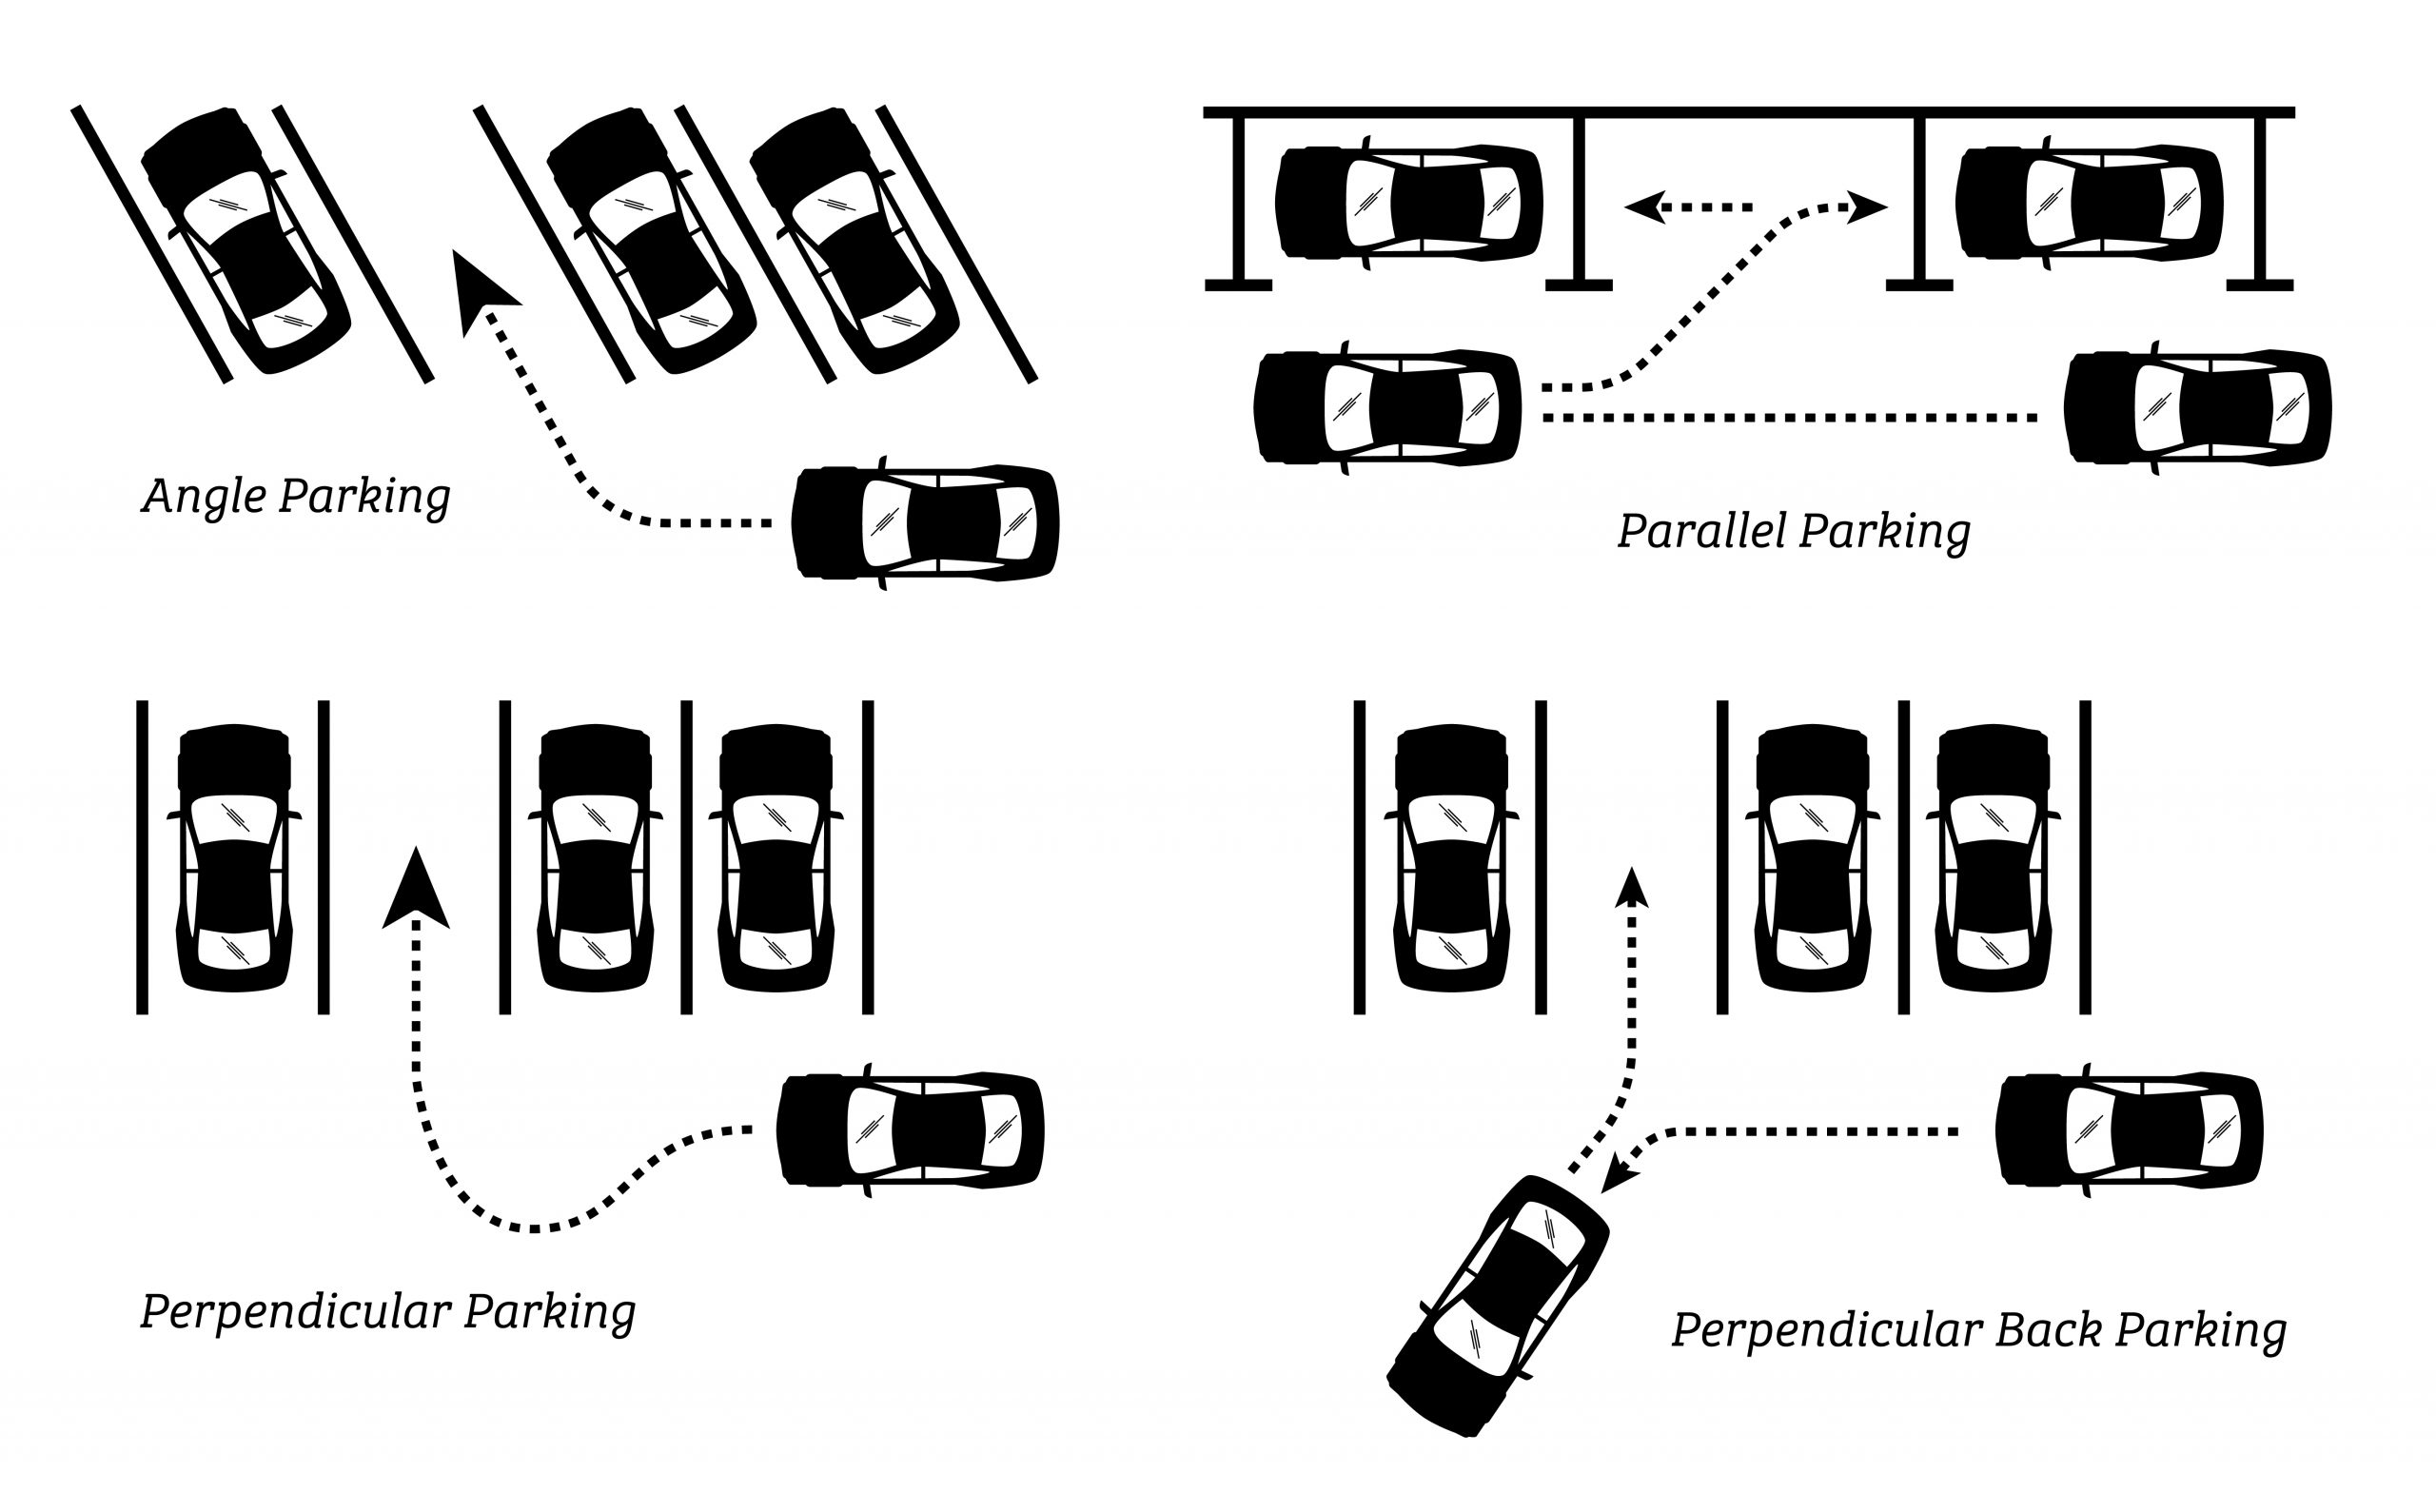
\includegraphics[width=4in]{images/Chap2/perpendicular-parking-a-lot-scaled.jpg}\\
    \caption{Parking Styles}
    \label{Parking Styles}
    \end{center}
\end{figure}

Analogically, after the truck arrives in the station, the drivers would drive and steer in the opposite direction of the 
pallet, until the forks are in a position to allow the truck to easily and correctfully drive to the pallet in fork direction.
The goal here is to develop a pallet-linking algorithm to automate the driving to the pallet pickup location for 
autonomous forklifts as given by figure \ref{pattern}. The truck would autonomously plan the path to its destination
based on the pattern and on the environment settings that it would navigate in. 
The pattern enhances the explainability in the forklifts behavior. Explainability allows for more order in the warehouse: 
it simplifies the coordination of safe simultaneous tasks around the truck. This is achieved through the design of an 
algorithm that aims to create a transparent navigation process, making it easier for humans to understand and trust 
the technology. Additionally, the approach is intended to ensure secure and reliable decision-making for autonomous trucks.



\begin{figure}
    [H]
    \begin{center}
    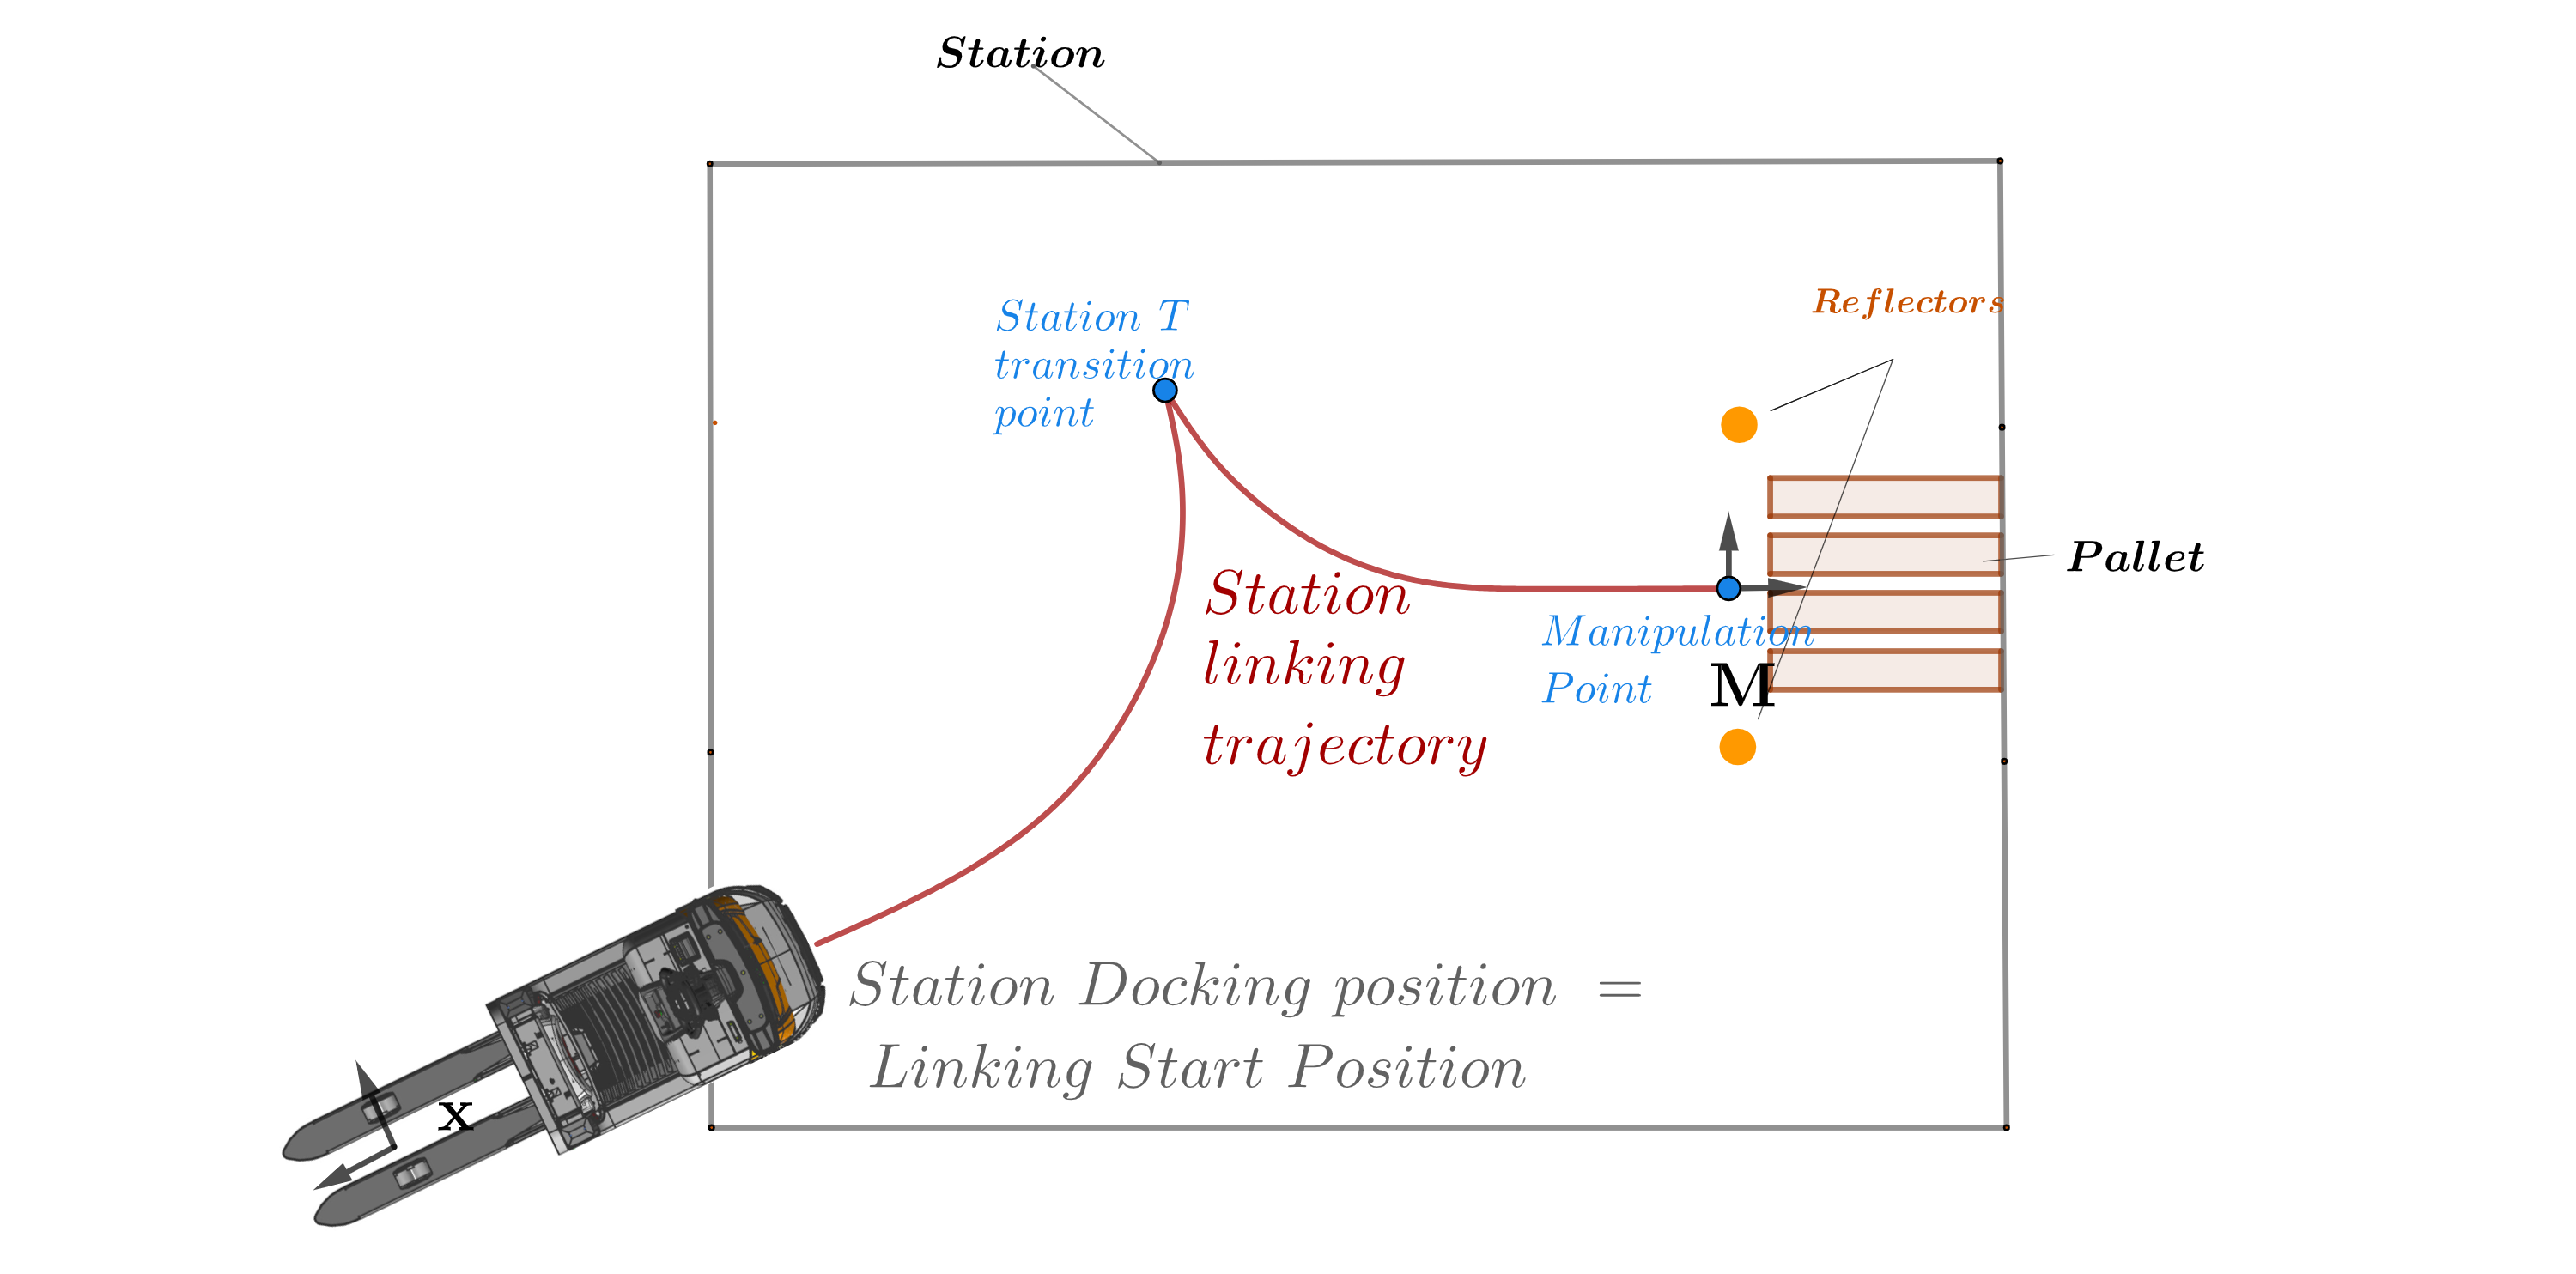
\includegraphics[width=\linewidth]{images/Chap2/station-without-subpolygones.png}\\
    \caption{Linking the robot to goal destination \cite{R28}}
    \label{pattern}
    \end{center}
\end{figure}
From now on, the following definitions of driving directions will be used as gven by figure \ref{driving directions}:
\begin{itemize}
    \item Main Driving Direction: Driving in fork direction.
    \item Opposite Driving Direction: Driving in vehicle chassis direction.
\end{itemize}

\begin{figure}
    [H]
    \begin{center}
    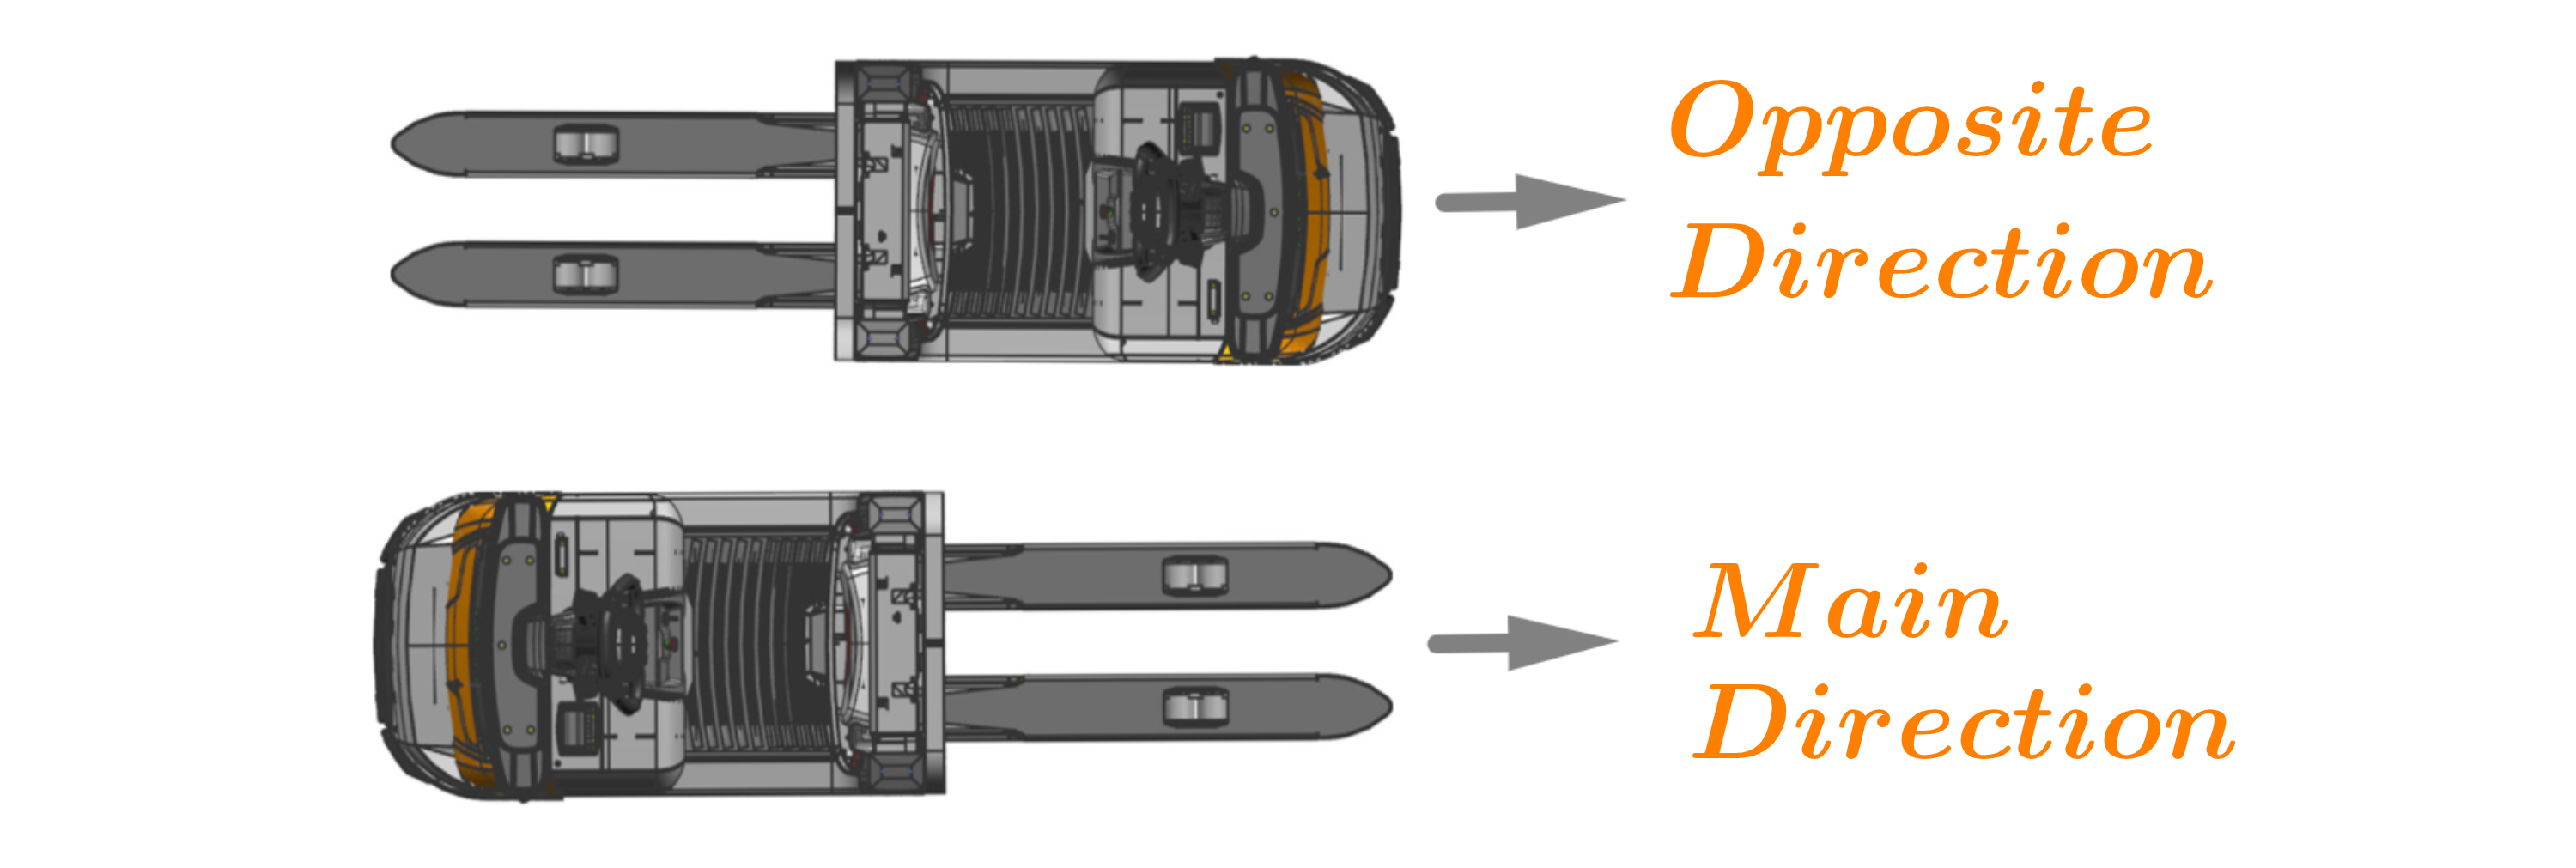
\includegraphics[width=4in]{images/Chap2/driving_directions.png}\\
    \caption{Truck Driving Directions}
    \label{driving directions}
    \end{center}
\end{figure} 
 
The following transition method is suggested: once the truck docks the station, it has the option to transition and change 
direction on the sides of the shelf placed inside the station. First, it drives to the transition position, then, to the 
pallet or the drop-off position as given by figure \Ref{subpolygones}. Having two possibilities for transition zones allows 
for more flexibility: 
in case one area is unreachable or presents obstacles, the second one can be used. They present free areas 
inside the stations where less obstacles and dynamics are expected and smooth maneuvering of the truck can be managed. 
In addition, the geometric solution is scalable to 
any station that is recognized and whose properties are available to the truck. This makes the overall solution and the 
autonomous forklifts simple to
commission in new warehouses.

\begin{figure}
    [H]
    \begin{center}
    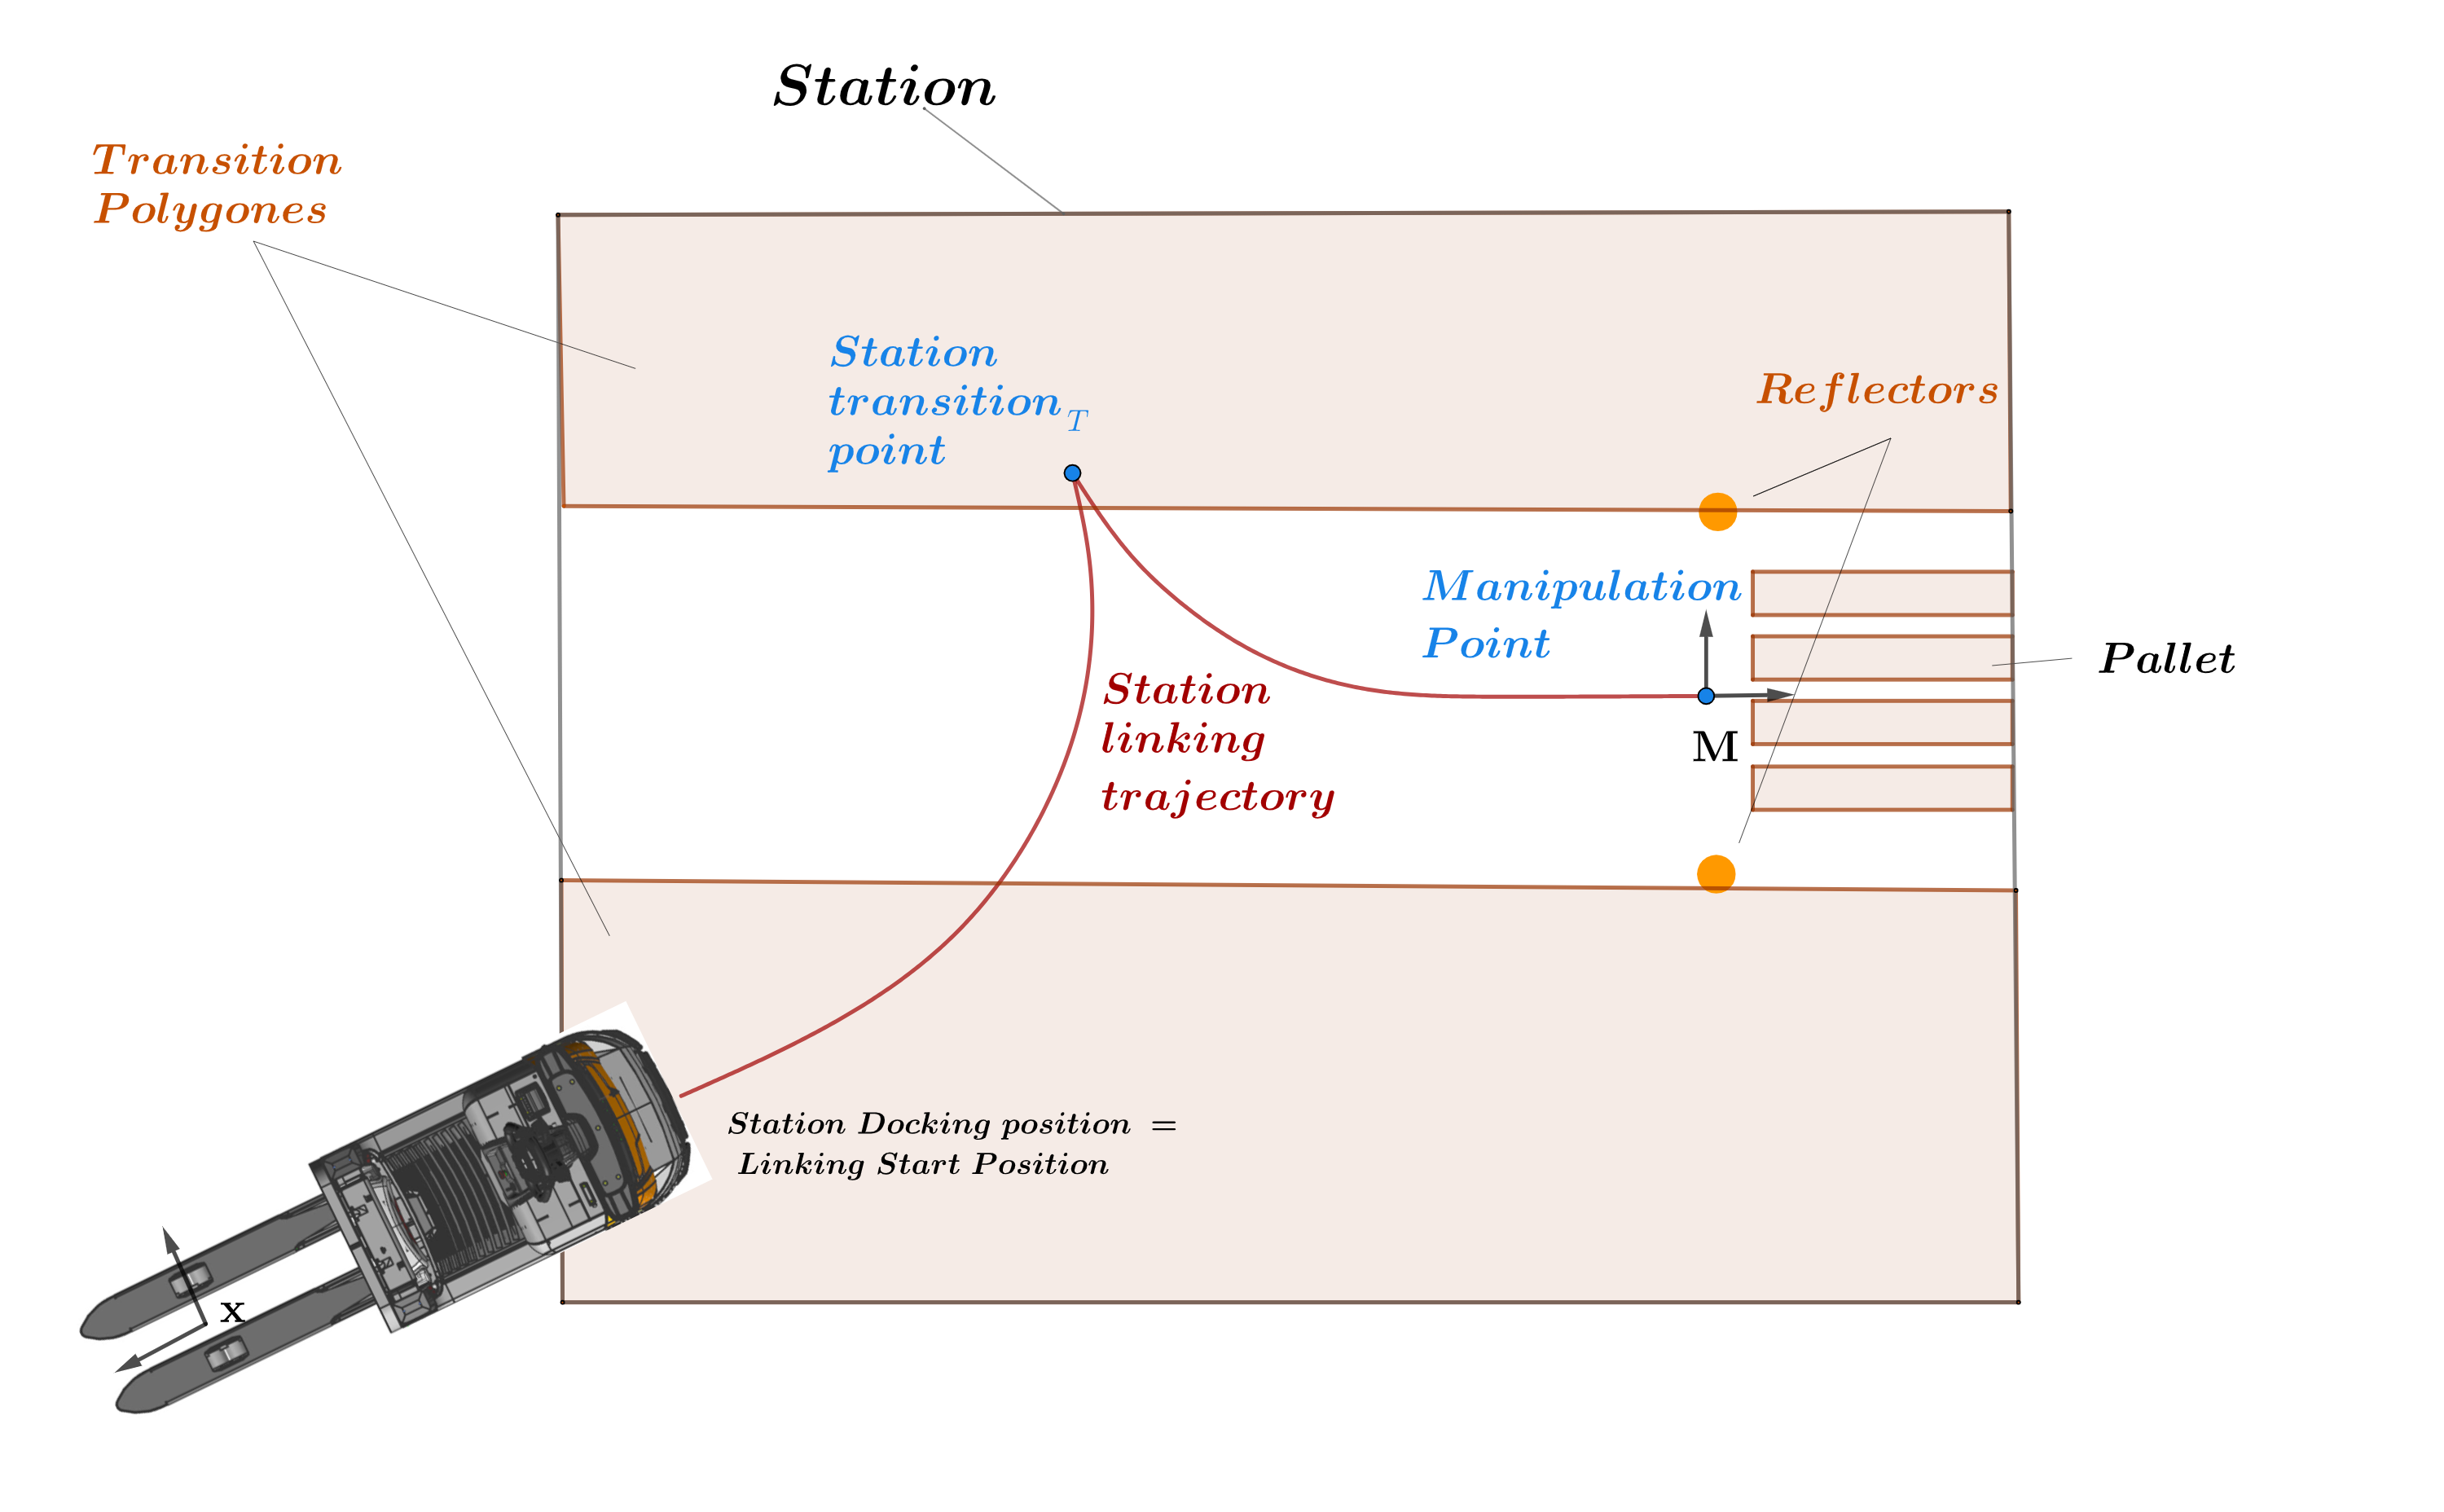
\includegraphics[width=\linewidth]{images/Chap2/station-without-subpolygones (2).png}\\
    \caption{Linking the robot to goal pallet \cite{R28}}
    \label{subpolygones}
    \end{center}
\end{figure}

Smooth and continuous paths are generated through spline interpolation of constructed waypoints. This technique ensures 
that the resulting paths are smooth, operationally seamless, and reduce abrupt changes in direction and speed. 
By interpolating between waypoints, the method enables the creation of curves that are optimized for driving efficiency 
and stability.

Finally, an optimizer generates an optimal path. 
generates multiple path candidates and rigorously evaluates each one based on key factors. 
The evaluation considers the path's length, smoothness, and potential collisions with surrounding objects to ensure the 
chosen path is both efficient and safe. After testing all options, the path that best meets these 
criteria—providing the shortest, smoothest, and safest route with minimal collision risk—is selected as the best solution. 

This approach ensures the final path is not only theoretically ideal but also practical and reliable for real-world use. 
The process is designed to be flexible and effective, even in obstacle environments. The designed methodology 
is summarized in the following flowchart \ref{design}:

\begin{figure}[!ht]
    \begin{center}
        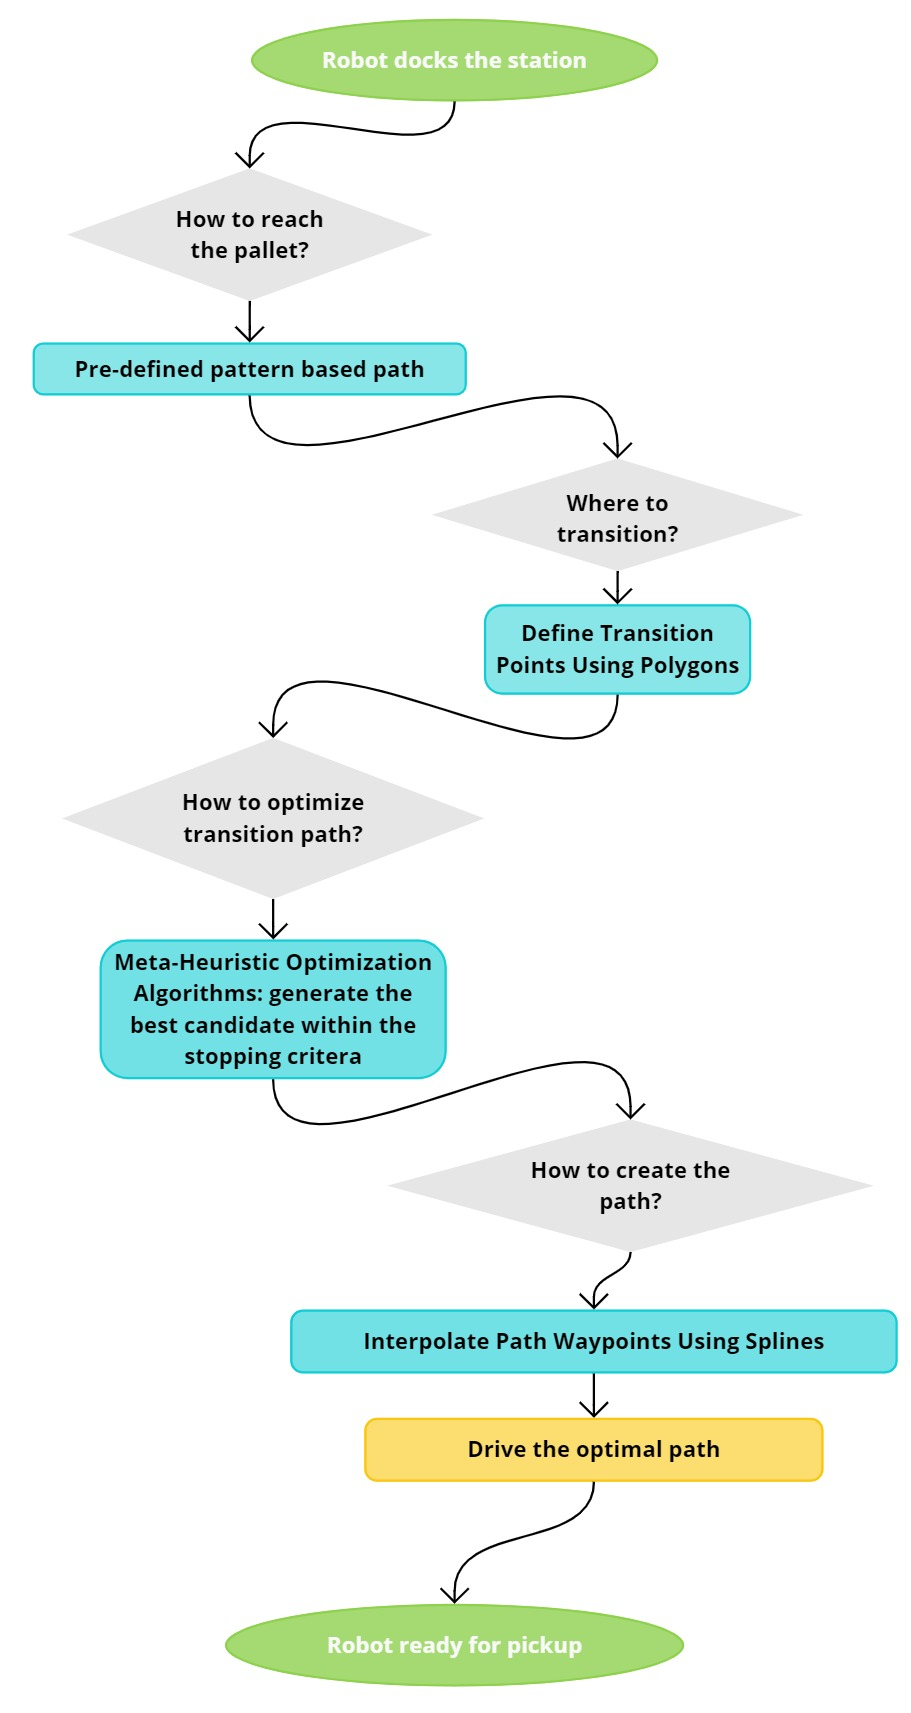
\includegraphics[width=4in]{images/Chap2/Approch_design.jpg}\\
        \caption{Path planning approach to pallet docking}
        \label{design}
        \end{center}
\end{figure}

